\documentclass{article}%
\usepackage[T1]{fontenc}%
\usepackage[utf8]{inputenc}%
\usepackage{lmodern}%
\usepackage{textcomp}%
\usepackage{lastpage}%
\usepackage[head=40pt,margin=0.5in,bottom=0.6in]{geometry}%
\usepackage{graphicx}%
%
\title{\textbf{Renuncia cardenal condenado por encubrir abusos en Francia}}%
\author{AP}%
\date{07/03/2019}%
%
\begin{document}%
\normalsize%
\maketitle%
\textbf{URL: }%
http://www.eluniversal.com/internacional/34988/francia{-}renuncia{-}cardenal{-}condenado{-}por{-}encubrir{-}abusos\newline%
%
\textbf{Periodico: }%
EU, %
ID: %
34988, %
Seccion: %
internacional\newline%
%
\textbf{Palabras Claves: }%
NO\_TIENE\newline%
%
\textbf{Derecho: }%
2.1%
, Otros Derechos: %
\newline%
%
\textbf{\textit{En una breve declaración a la prensa en Lyon, el cardenal francés Philippe Barbarin dijo que "he resuelto ir a ver al Santo Padre y ofrecerle mi renuncia" y que se reunirá con el papa "en unos días"}}%
\newline%
\newline%
%
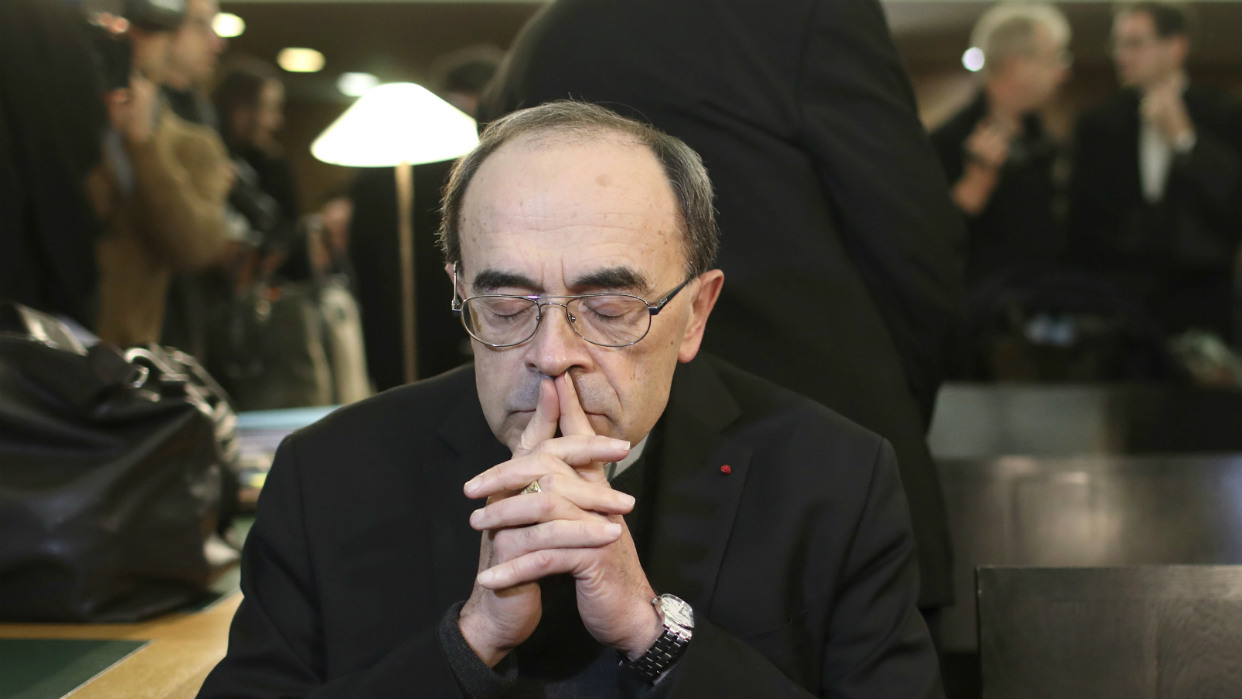
\includegraphics[width=300px]{EU_34988.jpg}%
\newline%
%
Lyon, Francia.{-} El cardenal francés Philippe Barbarin dijo el jueves que presentará su renuncia al papa Francisco tras ser condenado por encubrir a un cura pedófilo.%
\newline%
%
En una breve declaración a la prensa en Lyon, Barbarin dijo que "he resuelto ir a ver al Santo Padre y ofrecerle mi renuncia". Dijo que se reunirá con el papa "en unos días", indicó AP.%
\newline%
%
Barbarin expresó "compasión" por las presuntas víctimas y dijo que oraba por ellas.%
\newline%
%
Barbarin, la máxima autoridad católica en Francia, fue declarado culpable el jueves de no reportar a la justicia las acusaciones de presuntos abusos sexuales a menores por parte de un sacerdote pedófilo. Las víctimas consideran que la sorpresiva decisión es una victoria para la protección de los niños y una fuerte señal hacia la Iglesia.%
\newline%
%
El tribunal de Lyon sentenció a Barbarin a seis meses de prisión suspendida por no denunciar los hechos en el periodo comprendido entre julio de 2014 y junio de 2015.%
\newline%
%
Las supuestas víctimas del sacerdote Bernard Preynat dijeron que Barbarin y otras autoridades eclesiásticas encubrieron al cura durante años, pero algunas de las acusaciones habían prescrito e incluso las víctimas esperaban que el cardenal fuese absuelto. La fiscalía también se mostró contraria a una condena, alegando que no había motivos para demostrar una infracción legal.%
\newline%
%
Otros cinco acusados fueron absueltos.%
\newline%
%
Barbarin no estuvo presente en el tribunal el jueves pero su abogado, Jean{-}Felix Luciani, dijo que apelará el fallo.%
\newline%
%
"Esta es una decisión que no es justa a nivel jurídico", apuntó Luciani. "Esperamos que en el proximo nivel se haga justicia".%
\newline%
%
El Vaticano no respondió de inmediato a una petición de comentarios.%
\newline%
%
Preynat confesó haber abusado de miembros de los Boy Scouts en las décadas de 1970 y 1980 y será juzgado por separado.%
\newline%
%
Nueve personas que dijeron haber sufrido abusos por parte del religioso llevaron el caso contra Barbarin a los tribunales.%
\newline%
%
"Esta es una victoria que envía una fuerte señal a muchas víctimas y también a la Iglesia", manifestó François Devaux, presidente de la asociación "La Parole Liberee", que agrupa a víctimas de Preynat.%
\newline%
%
"Vemos que nadie está por encima de la ley. Hemos sido escuchados por el tribunal. Este es el final de un largo camino", agregó.%
\newline%
%
Un abogado que representa a algunas de las supuestas víctimas de Preynat, Yves Sauvayre, calificó el veredicto de "histórico".%
\newline%
%
"El cardenal está condenado porque no hizo lo que tenía hacer", afirmó.%
\newline%
%
Según las víctimas, altos cargos eclesiásticos estaban al tanto de las acciones del sacerdote desde 1991, pero le permitieron estar en contacto con menores hasta su retirada en 2015.%
\newline%
%
Además de Barbarin, en el banquillo se sentaron un arzobispo, un obispo, un cura y otros dos funcionarios. Otro alto cargo de la Iglesia, el cardenal Luis Ladaria, estaba acusado pero no compareció porque el Vaticano invocó su inmunidad diplomática.%
\newline%
%
\end{document}